\documentclass[aspectratio=169,
hyperref={colorlinks,urlcolor=blue}
]{beamer}


%\usetheme{Pittsburgh}
\usetheme{default}
\usepackage{colortbl}%colored tables
%For using helvetica font:
\usepackage[scaled]{helvet}
\usepackage[T1]{fontenc}
\renewcommand\familydefault{\sfdefault}
\urlstyle{same} %sets the fonts for urls
\usepackage{pdfpages}
\usepackage{siunitx}
\usepackage{caption}
\usepackage{pifont}%for dings
\usepackage{pgfplots}%for 3d plotting
\pgfplotsset{compat = newest}
\usepackage{mathtools}%box in align env \Aboxed
\usepackage[american,smartlabels]{circuitikz}%for drawing circuits
\usepackage{multimedia}
\usepackage{animate}
\usepackage{xcolor}


\usetikzlibrary{arrows}
\usetikzlibrary {3d} 
\usetikzlibrary{decorations.markings, math}
\usetikzlibrary{intersections, pgfplots.fillbetween}
\usetikzlibrary {shapes.geometric} 


%\definecolor{myblue}{RGB}{5, 34, 150}
\definecolor{myblue2}{RGB}{5, 34, 150}
\definecolor{myblue}{RGB}{0,36,82}
\definecolor{myred}{RGB}{207, 2, 13}
\definecolor{mygreen}{RGB}{0, 158, 11}
\definecolor{myyellow}{RGB}{220,220,0}
\definecolor{qblue}{RGB}{0,36,82}
\definecolor{qgold}{RGB}{250,189,15}
\definecolor{qred}{RGB}{185,14,49}
\definecolor{cblue}{rgb}{0.13, 0.67, 0.8}
\definecolor{corange}{rgb}{0.8, 0.34, 0.0}
\definecolor{cpurple}{rgb}{0.54, 0.29, 0.42}

%%%%%%%%%%%% General settings
\setbeamercolor{frametitle}{fg=black}
\setbeamercolor{title}{fg=black}
\setbeamercolor{author}{fg=myblue2}

\beamertemplatenavigationsymbolsempty %no navigation controls at bottom of slides
%\setbeamertemplate{footline}[frame number]
\usefonttheme{professionalfonts} 
\setbeamerfont{title}{series=\bfseries,parent=structure}
\setbeamerfont{frametitle}{series=\bfseries,parent=structure}

%%%%%%%%%%%%Lists
\setbeamertemplate{itemize item}[circle] %{\color{myblue}$\circ$}
\setbeamertemplate{itemize subitem}{\color{myblue2}$\circ$}
\setbeamertemplate{itemize subsubitem}{\color{myblue2}$\cdot$}
\setbeamercolor{itemize item}{bg=myblue2,fg=myblue2}
\setbeamercolor{enumerate item}{bg=myblue2,fg=myblue2}
%%%%%%%%%%%%%%%%%%%%%%%%%%%%

%%%%%%%%%%%%Blocks
\setbeamertemplate{blocks}[rounded]
%Default block
\setbeamercolor{block title}{bg=myblue2, fg=white}
\setbeamercolor{block body}{bg=myblue2!10}
\setbeamerfont{block body}{size=\scriptsize}
\setbeamerfont{block title}{size=\scriptsize}
%Alert block
\setbeamercolor{block title alerted}{bg= myblue2, fg=white}
\setbeamercolor{block body alerted}{bg=myblue2!10}
\setbeamerfont{block body alerted}{size=\scriptsize}
\setbeamerfont{block title alerted}{size=\scriptsize}
%example block
\setbeamercolor{block title example}{bg=mygreen, fg=white}
\setbeamercolor{block body example}{bg=mygreen!10}
\setbeamerfont{block body example}{size=\scriptsize}
\setbeamerfont{block title example}{size=\scriptsize}
%%%%%%%%%%%%%%%%55


%%%%%%%%%%%%Figures and captions
\captionsetup{font=scriptsize,labelfont=scriptsize}
%\setbeamertemplate{caption}{\raggedright\insertcaption\par}
\newenvironment{capfig}[3]{\begin{figure}\includegraphics[width=#1\textwidth]{#2}\caption*{\textit{#3}}\end{figure}}{}

%\makeatother
%\setbeamertemplate{footline}
%{
%  \leavevmode%
%  \hbox{%
%  \begin{beamercolorbox}[wd=.4\paperwidth,ht=2.25ex,dp=1ex,center]{author in head/foot}%
%    \usebeamerfont{author in head/foot}\insertshortauthor
%  \end{beamercolorbox}%
%  \begin{beamercolorbox}[wd=.6\paperwidth,ht=2.25ex,dp=1ex,center]{title in head/foot}%
%    \usebeamerfont{title in head/foot}\insertshorttitle\hspace*{3em}
%    \insertframenumber{} / \inserttotalframenumber\hspace*{1ex}
%  \end{beamercolorbox}
%  }%
%  \vskip0pt%
%}
%\makeatletter

\makeatother
\setbeamertemplate{footline}
{
  \leavevmode%
  \hbox{%
\begin{beamercolorbox}[wd=.27\paperwidth,ht=2.25ex,dp=1ex,center]{author in head/foot}%
    \color{black}{\insertinstitute}
\end{beamercolorbox}
  \begin{beamercolorbox}[wd=.27\paperwidth,ht=2.25ex,dp=1ex,center]{author in head/foot}%
    \color{black}{\inserttitle}
  \end{beamercolorbox}%
  \begin{beamercolorbox}[wd=.27\paperwidth,ht=2.25ex,dp=1ex,center]{title in head/foot}%
    \color{black}{\insertshortauthor}
  \end{beamercolorbox}
  \begin{beamercolorbox}[wd=.27\paperwidth,ht=2.25ex,dp=1ex,center]{title in head/foot}%
    \hspace{.28\paperwidth}\color{black} \insertframenumber{} / \inserttotalframenumber\hspace*{1ex}
  \end{beamercolorbox}
  }%
  \vskip0pt%
}
\makeatletter

\setbeamertemplate{title page}
{
  \begin{tikzpicture}[remember picture,overlay]
    \def\barh{4}%15
  
    \draw[color=myblue2,line width=\barh] ([yshift=-0.5*\barh]current page.north west) -- ([yshift=-0.5*\barh,xshift=-0.67\paperwidth]current page.north east);
    \draw[color=myblue2,line width=\barh] ([yshift=-0.5*\barh,xshift=-0.67\paperwidth]current page.north east) -- ([yshift=-0.5*\barh,xshift=-0.34\paperwidth]current page.north east);
    \draw[color=myblue2,line width=\barh] ([yshift=-0.5*\barh,xshift=-0.34\paperwidth]current page.north east) -- ([yshift=-0.5*\barh]current page.north east); 
  
    \draw[color=myblue2,line width=\barh] ([yshift=0.5*\barh]current page.south west) -- ([yshift=0.5*\barh,xshift=-0.67\paperwidth]current page.south east);
    \draw[color=myblue2,line width=\barh] ([yshift=0.5*\barh,xshift=-0.67\paperwidth]current page.south east) -- ([yshift=0.5*\barh,xshift=-0.34\paperwidth]current page.south east);
    \draw[color=myblue2,line width=\barh] ([yshift=0.5*\barh,xshift=-0.34\paperwidth]current page.south east) -- ([yshift=0.5*\barh]current page.south east);
    %\node[left] at (current page.east) {
    %
\includegraphics[scale=0.1]{figures/coverpage}
    %};
  \end{tikzpicture}
  
  \usebeamerfont{title}\usebeamercolor[fg]{title}\inserttitle\par
  \usebeamerfont{subtitle}\usebeamercolor[fg]{subtitle}\insertsubtitle\par
  \vspace{2cm}
  \usebeamerfont{author}\usebeamercolor[fg]{author}\insertauthor\par
  \usebeamerfont{institute}\usebeamercolor[fg]{author}\insertinstitute\par
  \usebeamercolor[fg]{author}\par
  \usebeamercolor[fg]{titlegraphic}\inserttitlegraphic

} 

\setbeamertemplate{frametitle}{%
    \nointerlineskip%
        \par\hspace*{-\dimexpr0.5\paperwidth-0.5\textwidth}\textcolor{myblue2}{\rule{0.33\paperwidth}{6pt}}\textcolor{myblue2}{\rule{0.33\paperwidth}{6pt}}\textcolor{myblue2}{\rule{0.34\paperwidth}{6pt}} 
    \begin{beamercolorbox}[wd=\paperwidth,ht=0.75cm,dp=0.6ex]{frametitle}
        \hspace*{0.5cm}\strut\usebeamerfont{frametitle}\insertframetitle\strut
        %\hrule
    \end{beamercolorbox}%
    %%Line below:
%\par\hspace*{-\dimexpr0.5\paperwidth-0.5\textwidth}\textcolor{myblue}{\rule{\paperwidth}{0.4pt}}
     % <-- calculation of left margin width + rule
     %\textcolor{red}{\noindent\rule{\paperwidth}{2pt}}
}


%%%%%%%%%%%%Frame templates

%Slide with title
\newenvironment{titleframe}[1]
{\begin{frame}\frametitle{#1}\end{frame}}
{}

%Slide with title and itemize list:
\newenvironment{bulletframe}[1]
{\begin{frame}{#1} \itemize}
{\enditemize \end{frame}}

%Slide with two columns 50/50
\newenvironment{twocolframe}[3]
{\begin{frame}{#1}
 \begin{columns}[T]
 \column{0.5\textwidth}#2
 \column{0.5\textwidth}#3
 \end{columns}\end{frame}}{}

%Slide with two columns 60/40 <<<<<<<<<<<<<<<<<<<<<<  This one!
\newenvironment{twocolframesf}[3]
{\begin{frame}{#1}
 \begin{columns}[T]
 \column{0.6\textwidth}#2
 \column{0.4\textwidth}#3
 \end{columns}\end{frame}}{}
 
%Slide with two columns 70/30
\newenvironment{twocolframest}[3]
{\begin{frame}{#1}
 \begin{columns}[T] 
 \column{0.7\textwidth}#2
 \column{0.3\textwidth}#3
 \end{columns}\end{frame}}{} 
 
%Slide with two columns 40/60
\newenvironment{twocolframefs}[3]
{\begin{frame}{#1}
 \begin{columns}[T] 
 \column{0.4\textwidth}#2
 \column{0.6\textwidth}#3
 \end{columns}\end{frame}}{}
 
%Slide with two columns 70/30
\newenvironment{twocolframets}[3]
{\begin{frame}{#1}
 \begin{columns}[T] 
 \column{0.3\textwidth}#2
 \column{0.7\textwidth}#3
 \end{columns}\end{frame}}{} 

 
%Colloquium speaker (title, abstract, picture file, speaker name)
\newenvironment{colloquium}[5]
{
\begin{frame}{Colloquium: Friday 1:30pm in Stirling A}
\begin{columns}[T] 
 \column{0.8\textwidth}
 \textbf{#1}\\
 #2
 \column{0.2\textwidth}
 \capfig{#3}{#4}{#5}
 \end{columns}
\end{frame}
}
{} 

%%%%%%%%%%%%%Set Hyperref colors


\hypersetup{
  colorlinks=true,
  linkcolor=blue,    
  urlcolor=blue,     
  citecolor=blue      
}
%%%%%%%%%%%%%TOC bolding
\setbeamerfont{section in toc}{series=\bfseries}



%Frames:
% \twocolframesf 60/40 (fs, st, ts) 
% \titleframe
% bulletframe


%%%%%%%%%%%%%%%%%%%%%%%%%
%%%%%% START OF PRESENTATION %%%%%%
%%%%%%%%%%%%%%%%%%%%%%%%%

\title{Potential \& Conservation of Energy}
\subject{Conservation, Potential and Potential Uses}
\subtitle{Building Models to Describe our World}


\begin{document}

%%%%%%%%%%%%%%%%%%%%%%%%%
%%%%%% Title slide %%%%%%
%%%%%%%%%%%%%%%%%%%%%%%%%
\chaptertitle{Potential \& Conservation of Energy}
\begin{frame}
\titlepage
\thispagestyle{empty}

\begin{textblock*}{5cm}(11cm,4cm)
    
\includegraphics[width=4cm]{figures/BMDW/logo}
\end{textblock*}

\end{frame}

%%%%%%%%%%%%%%%%%%%%%%%%%%%%%%%%%





\twocolframe{Outline}
{\tableofcontents[sections=1, subsectionstyle=show/show]\thispagestyle{empty}}
{\tableofcontents[sections=2-3, subsectionstyle=show/show]}






%%%%%%%%%%%%%%%%%%%%%%%%%%%%%%%%%%%%%%%

\section{Conservative Forces}
\label{sec:conservativeforces}
\title{Conservative Forces}
\institute{Conservation, Potential and Potential Uses}
\author{\insertsubsection}


%%%%%%%%%%%%%%%%%%%%%%%%%
\begin{frame}
\titlepage
\thispagestyle{empty}
\end{frame}

%%%%%%%%%%%%%%%%%%%%%%%%




\subsection{Work Recap}
\label{subsec:workrecap}
\twocolframesf{Recall: Work}
{
\begin{align*}
W=\int_A^B \vec F(\vec r) \cdot d\vec l
\end{align*}
\begin{itemize}
\item Force can change magnitude and direction based on position.
\item Need to define work as a ``path integral'', as it depends on the path taken.
\item In general, this integral can be difficult to evaluate.
\end{itemize}
}
{
\vspace{-1cm}
\begin{center}
\begin{tikzpicture}[%
%https://tex.stackexchange.com/questions/25928/how-to-draw-tangent-line-of-an-arbitrary-point-on-a-path-in-tikz
        tangent/.style={
        decoration={
            markings,% switch on markings
            mark=
                at position ####1
                with
                {
                    \coordinate (tangent point-\pgfkeysvalueof{/pgf/decoration/mark info/sequence number}) at (0pt,0pt);
                    \coordinate (tangent unit vector-\pgfkeysvalueof{/pgf/decoration/mark info/sequence number}) at (1,0pt);
                    \coordinate (tangent orthogonal unit vector-\pgfkeysvalueof{/pgf/decoration/mark info/sequence number}) at (0pt,1);
                }
        },
        postaction=decorate
    },
    use tangent/.style={
        shift=(tangent point-####1),
        x=(tangent unit vector-####1),
        y=(tangent orthogonal unit vector-####1)
    },
    use tangent/.default=1
    ]
\tikzmath{
}

\scalebox{0.8}{

 \coordinate (P1) at (0.2,0.5);
 \coordinate (P2) at (1.75,2); %used to make the path squiggly
 \coordinate (P3) at (3.75,2.5);
 \coordinate (P3x) at ($(0,0)!(P3)!(1,0)$);
 \coordinate (P1P3) at ($(P3)!(P1)!(P3x)$);
 
 \draw[-latex, line width=1.5pt] (0,0) -- (4.5,0) node[below]{$x$}; 
 \draw[-latex, line width=1.5pt] (0,0) -- (0,3) node[left]{$y$}; 
 
 \fill (P1) circle(2pt) node[above]{$A$};;
 \fill (P3) circle(2pt) node[above]{$B$};;
 
  
 %The path with tangent coordinates calculated
 \draw[tangent=0.25,tangent=0.45,tangent=0.65, tangent=0.85,  line width=1pt] (P1) to [out=10,in=190] (P2) to [out=10,in=260] (P3);
 
 \draw [myred, -latex, line width=1.5, use tangent=2] (-0.25,0) -- (0.25,0) node[above]{$d\vec l$};
 %\draw [ -latex, line width=1.5, use tangent=2] (0,0) -- +(-60:1) node[right]{$\vec F(\vec r)$}; 
 \draw [ -latex, line width=1.5, use tangent=1] (0,0) -- +(-80:0.75) node[below]{$\vec F(\vec r)$}; 
 %\draw [ -latex, line width=1.5, use tangent=3] (0,0) -- +(60:1.25) node[above]{$\vec F(\vec r)$}; 
 
 \begin{scope}[shift={(0,-3.5)}]
 
 \coordinate (A) at (0.75,0.5);
 \coordinate (B) at (3.75,2.5);
 
 
 \draw[-latex, line width=1.5pt] (0,0) -- (4.5,0) node[below]{$x$}; 
 \draw[-latex, line width=1.5pt] (0,0) -- (0,3) node[left]{$y$}; 

 \fill (A) circle(2pt) node[right]{$A(x_A,y_A)$};
 \fill (B) circle(2pt) node[above]{$B(x_B,y_B)$};
 
 \draw[dashed, line width=1.5] (A)--(B) node[midway,right=5pt]{path 1};
 
 \draw[-latex, color=myred, line width=1.5pt] (A)-- +(0,2.0)node[midway,left]{$\vec d_1$} node[above]{path 2};
 \draw[latex-, color=myred, line width=1.5pt] (B)-- +(-3,0) node[midway,above]{$\vec d_2$};
 
 \draw[latex-, line width=3] (1,1) -- +(0,1) node[midway, right]{$\vec f_1$};
 \draw[-latex, line width=3] (2.5,2.25) -- +(-1,0) node[midway, below]{$\vec f_2$};
 
 
 \end{scope} 
 
}
\end{tikzpicture}
\captionof*{figure}{\textit{Work is a path integral.}}
\end{center}
}


%%%%%%%%%%%%%%%%%%%%%%%%%%%%%%%%
\twocolframest{Recall: Work-Energy Theorem}
{
\only<1>{
\begin{itemize}
\item The net work done on an object is its change in kinetic energy:
\begin{align*}
W^{net}=\Delta K
\end{align*}
\end{itemize}}
\only<2>{
\begin{exampleblock}{Example: Object falling due to gravity}
The work done by gravity:
\begin{align*}
W^{net}=\vec F_g \cdot \vec d = mgh
\end{align*}
The change in kinetic energy (final - initial)
\begin{align*}
\Delta K = \frac{1}{2}mv^2-0=\frac{1}{2}mv^2
\end{align*}
Work-Energy theorem:
\begin{align*}
W^{net}&=\Delta K\\
mgh &=\frac{1}{2}mv^2\\
\therefore v&=\sqrt{2gh}
\end{align*}
\end{exampleblock}
}
}
{
\only<2>{
\begin{center}
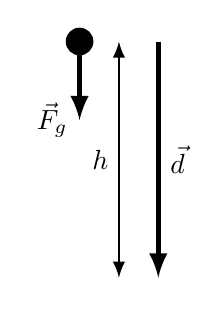
\begin{tikzpicture}
\tikzmath{
\h=3;
}

\scalebox{1}{
\fill (0,0) circle(5pt);
\draw [-latex,line width=2] (0,0) -- +(0,-1) node[left]{$\vec F_g$};
\draw [latex-latex,line width=1] (0.5,0) -- +(0,-\h) node[midway,left]{$h$}; 
\draw [-latex,line width=2] (1,0) -- +(0,-\h) node[midway,right]{$\vec d$}; 
}
\end{tikzpicture}
\captionof*{figure}{\textit{A mass, $m$, falls a distance, $h$, with a corresponding displacement, $\vec d$.}}
\end{center}}

}


%%%%%%%%%%%%%%%%%%%%%%%%%%%%%%%%
\subsection{Conservative vs non-conservatice forces}
\label{subsec:conservativevsnonconservativeforces}
\begin{frame}{Conservative vs non-conservative forces}
\begin{itemize}
\item A non-conservative force is one for which the work done depends on the path taken.
\item A conservative force is one for which the work done does not depend on the path taken:
\begin{itemize}
\item Corollary: The work done by a conservative force along a closed path is zero.
\end{itemize}
\end{itemize}
\end{frame}


%%%%%%%%%%%%%%%%%%%%%%%%%%%%%%%%


%%%%%%%%%%%%%%%%%%%%%%%%%%%%%%%%
\subsubsection{Condition for a force to be conservative}
\label{subsec:conditionforconservativeforce}
\begin{frame}{Condition for a force to be conservative}
\begin{itemize}
\item The work done on a closed path must be zero:
\begin{align*}
W=\textcolor{myred}{\int_A^A}\vec F(\vec r) \cdot d\vec l = \textcolor{myred}{\oint}\vec F(\vec r) \cdot d\vec l = 0
\end{align*}
\item This requires the following conditions on, $\vec F(\vec r)$, (given by Stokes' Theorem, which is way beyond the scope of this course):
\begin{align*}
\frac{\partial F_z}{\partial y}-\frac{\partial F_y}{\partial z}&=0\\
\frac{\partial F_x}{\partial z}-\frac{\partial F_z}{\partial x}&=0\\
\frac{\partial F_y}{\partial x}-\frac{\partial F_x}{\partial y}&=0
\end{align*}
... evaluating these partial derivatives is however not beyond the scope of this course!
\end{itemize}
\end{frame}


%%%%%%%%%%%%%%%%%%%%%%%%%%%%%%%%
\begin{frame}{Example of a conservative force}
\begin{itemize}
\item The force from a spring:
\begin{align*}
\vec F(\vec r)=\vec F(x,y,z)=F_x \hat x+F_y\hat y+F_z\hat z = -kx\hat x+0\hat y+0\hat z
\end{align*}
\item Take one of the terms:
\begin{align*}
\frac{\partial F_x}{\partial z}-\frac{\partial F_z}{\partial x}=\frac{\partial}{\partial z}( -kx)-\frac{\partial}{\partial x}0=0
\end{align*}
\item They are all zero $\rightarrow$ The force from a spring is conservative !
\end{itemize}
\end{frame}


%%%%%%%%%%%%%%%%%%%%%%%%%%%%%%%%
\subsubsection{Work by a conservative force}
\label{subsubsec:workbyaconservativeforce}
\twocolframesf{Work by a conservative force – Potential energy}
{
\begin{itemize}
\item The work done by a conservative force does not depend on the path, only on the end points:
\begin{align*}
W=\int_A^B \vec F(\vec r) \cdot d\vec l
\end{align*}
\item We introduce a \textbf{function of position}, $U(\vec r)$ , such that the \textbf{negative of the work} done by the conservative force can be calculated using that function:
\begin{align*}
-W=-\int_A^B \vec F(\vec r) \cdot d\vec l=U(\vec r_B)-U(\vec r_A)=\Delta U
\end{align*}
\end{itemize}
}
{
\vspace{-1cm}
\begin{center}
\begin{tikzpicture}[%
%https://tex.stackexchange.com/questions/25928/how-to-draw-tangent-line-of-an-arbitrary-point-on-a-path-in-tikz
        tangent/.style={
        decoration={
            markings,% switch on markings
            mark=
                at position ####1
                with
                {
                    \coordinate (tangent point-\pgfkeysvalueof{/pgf/decoration/mark info/sequence number}) at (0pt,0pt);
                    \coordinate (tangent unit vector-\pgfkeysvalueof{/pgf/decoration/mark info/sequence number}) at (1,0pt);
                    \coordinate (tangent orthogonal unit vector-\pgfkeysvalueof{/pgf/decoration/mark info/sequence number}) at (0pt,1);
                }
        },
        postaction=decorate
    },
    use tangent/.style={
        shift=(tangent point-####1),
        x=(tangent unit vector-####1),
        y=(tangent orthogonal unit vector-####1)
    },
    use tangent/.default=1
    ]
\tikzmath{
}

\scalebox{1}{

 \coordinate (P1) at (1,1.5);
 \coordinate (P2) at (1.75,2); %used to make the path squiggly
 \coordinate (P3) at (3.75,3);

 \draw[color=myblue!60,-latex, line width = 1.5] (0,0) -- (P1) node[midway, above=5pt,left=-4pt]{$\vec r_A$};
  \draw[color=myblue!60,-latex, line width = 1.5] (0,0) -- (P3) node[midway, below]{$\vec r_B$};
  
 \draw[-latex, line width=1.5pt] (0,0) -- (4.5,0) node[below]{$x$}; 
 \draw[-latex, line width=1.5pt] (0,0) -- (0,3) node[left]{$y$}; 
 
 \fill (P1) circle(2pt) node[right]{$A$};;
 \fill (P3) circle(2pt) node[right]{$B$};;
 
 \node[above=8pt,left=-5pt] at (P1) {$U(\vec r_A)$};
  \node[above] at (P3) {$U(\vec r_B)$};
  
 %The path with tangent coordinates calculated
 \draw[tangent=0.25,tangent=0.45,tangent=0.65, tangent=0.85,  line width=2pt] (P1) to [out=10,in=190] (P2) to [out=10,in=260] (P3);
 
 \draw [myred, -latex, line width=1.5, use tangent=3] (-0.25,0) -- (0.25,0) node[below]{$d\vec l$};
 \draw [ -latex, line width=1.5, use tangent=2] (0,0) -- +(80:0.75) node[above]{$\vec F(\vec r)$}; 

 
}
\end{tikzpicture}
\captionof*{figure}{\textit{Work done by a conservative force depends only on the end points.}}
\end{center}
$U(\vec r)$ is called the \textbf{potential energy function}. It is associated with a specific conservative force and \textbf{depends only on position}.
}


%%%%%%%%%%%%%%%%%%%%%%%%%%%%%%%%
\subsection{Example: potential energy for a spring}
\label{subsec:potentialenergyspringexample}
\twocolframesf{Example: Potential energy for a spring}
{
\begin{itemize}
\item We want to know the potential energy function for a spring. We start with Work:
\begin{align*}
-W=-\int_A^B\vec F(\vec r) \cdot \textcolor{myred}{d\vec l}=U(\vec r_B) - U(\vec r_A)
\end{align*}
\item<2-> Work from the spring in going from $A$ ($x=-d$) to $B$ ($x=0$):
\begin{align*}
-W=-\int_{-d}^0 -kx\hat x \cdot \textcolor{myred}{dx\hat x}=\int_{-d}^0kxdx=\frac{1}{2}k0^2-\frac{1}{2}kd^2
\end{align*}
\item<3-> Identify:
\begin{align*}
U(x)=\frac{1}{2}kx^2+C
\end{align*}
\end{itemize}
}
{
\begin{center}
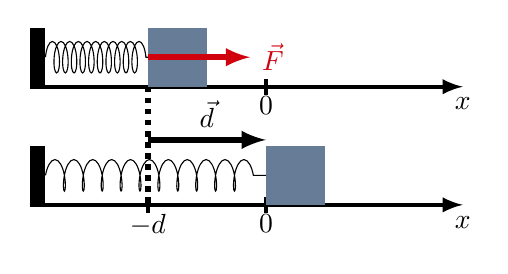
\begin{tikzpicture}[scale=1]
\tikzmath{
\L=2.;
\dx=0.75*\L;
\off=0.5;
\h=0.75;
}
\scalebox{1}{

\begin{scope}[shift={(0,-2*\h)}]
\draw[-latex,line width=1.5pt] (-1.5*\L,0) -- (1.25*\L,0) node[below]{$x$};
\draw[line width=1.5pt] (0,-0.1) -- (0,0.1);
\node[below] at (0,0) {$0$};

\fill (-1.5*\L,0) rectangle (-1.4*\L,\h);
\draw[decoration={aspect=0.3, segment length=2.4mm, amplitude=2mm,coil},decorate] (-1.4*\L,\h/2) -- (0,\h/2);
%\draw [latex-latex] (-1.4*\L,\h) -- (0,\h) node[midway,above]{$L_0$};
\fill[color=myblue!60] (0,0) rectangle (\h,\h);
\draw [-latex, line width=2] (-\dx,1.1*\h) -- (0,1.1*\h) node[midway,above]{$\vec d$};
 \node[below] at (-\dx,0) {$-d$};
 \draw[line width=1.5pt] (-\dx,-0.1) -- (-\dx,0.1);
\end{scope}
%%%%%%%%%%   compressed

\draw[-latex,line width=1.5pt] (-1.5*\L,0) -- (1.25*\L,0) node[below]{$x$};
\draw[line width=1.5pt] (0,-0.1) -- (0,0.1);
\node[below] at (0,0) {$0$};

\fill (-1.5*\L,0) rectangle (-1.4*\L,\h);
\draw[decoration={aspect=0.3, segment length=1.1mm, amplitude=2mm,coil},decorate] (-1.4*\L,\h/2) -- (-\dx,\h/2);

\fill[color=myblue!60] (-\dx,0) rectangle (-\dx+\h,\h);
\draw[line width=2, -latex,color=myred] (-\dx,\h/2) -- +(1.3,0) node[right] {$\vec F$};
\draw[dotted,line width=2] (-\dx,0) -- +(0,-2*\h);

}
\end{tikzpicture}
\vspace{-0.2cm}
\captionof*{figure}{\textit{Work done by a spring force,$\vec F(x)=-kx \hat x$ , from $x=-d$ to $x=0$. }}
\end{center}
\only<3>{
\textcolor{myred}{We can only determine potential energy up to a constant, since \textbf{only the difference in $U(x)$ is related to work}. Like an anti-derivative...} 
}
}


%%%%%%%%%%%%%%%%%%%%%%%%%%%%%%%%
\subsection{Work-energy and potential energy}
\label{subsec:workenergyandpotentialenergy}
\begin{frame}{Work-Energy Theorem and potential energy}
\begin{itemize}
\item The net work done can be  split into the sum of work done by conservative and non-conservative forces:
\begin{align*}
W^{net}=W^{NC}+W^{C}=\Delta K
\end{align*}
\item Re-arrange:
\begin{align*}
W^{NC}=\Delta K \textcolor{myred}{-}W^C
\end{align*}
\item Use potential energy for work done by conservative force:
\begin{align*}
W^{NC}=\Delta K \textcolor{myred}{+}\Delta U
\end{align*}
\item<2> This is why we introduced a minus sign when defining change in potential energy as the negative of work done, $\textcolor{myred}{-}W=\Delta U$.
\end{itemize}
\end{frame}


%%%%%%%%%%%%%%%%%%%%%%%%%%%%%%%%
\begin{frame}{Interpretation}
\begin{itemize}
\item The work done by non-conservative forces will change the ``energy'' (potential + kinetic) in the system:
\begin{align*}
W^{NC}=\Delta K +\Delta U=\Delta E
\end{align*}
\item Work done by non-conservative forces can \textit{add or remove} energy from the system:
\begin{itemize}
\item You push on a crate (do positive work), that energy goes into kinetic energy of the crate and/or (say) gravitational potential energy (if you push the crate up an incline).
\item A crate slides down an incline, the (negative) work done by friction removes energy, so the crate will have less kinetic energy than it otherwise would have.

\end{itemize}

\end{itemize}
\end{frame}


%%%%%%%%%%%%%%%%%%%%%%%%%%%%%%%%
\subsection{Force from potentital energy}
\label{subsec:forcefrompotentialenergy}
\begin{frame}{Force from potential energy (e.g. for a spring)}
\begin{itemize}
\item Effectively, the \textbf{potential energy can be found from the anti-derivative} of a force function (if we take the path integral on a path parallel to the direction of the force):
\begin{align*}
-W=-\int_{-d}^0 F(x) dx=\int_{-d}^0 kxdx=\frac{1}{2}k0^2-\frac{1}{2}kd^2=U(0)-U(-d)
\end{align*}
where we easily identified $U(x)=\frac{1}{2}kx^2+C$.
\item The force can then be found from the derivative of the potential energy function:
\begin{align*}
F(x)=-\frac{dU}{dx}=-\frac{d}{dx}\left(\frac{1}{2}kx^2+C\right)=-kx
\end{align*}
The signs matter, be careful!
\end{itemize}
\end{frame}


%%%%%%%%%%%%%%%%%%%%%%%%%%%%%%%%
\begin{frame}{Force from potential energy in 3D}
\begin{itemize}
\item In 3D, the potential energy is a \textbf{scalar function} of space, $U(x,y,z)$. 
\item The force \textbf{vector} is given by the negative of the \textbf{gradient vector} of the potential energy function (which you find with the partial derivatives):
\begin{align*}
\vec F &= -\nabla U(x,y,z)\\
F_x&=-\frac{\partial}{\partial x}U(x,y,z)\\
F_y&=-\frac{\partial}{\partial y}U(x,y,z)\\
F_z&=-\frac{\partial}{\partial z}U(x,y,z)
\end{align*}
\end{itemize}
\end{frame}


%%%%%%%%%%%%%%%%%%%%%%%%%%%%%%%%













%%%%%%%%%%%%%%%%%%%%%%%%%%%%%%%%

\section{Conservation of Energy}
\label{sec:conservationofenergy}
\title{Conservation of Energy}
\institute{Conservation, Potential and Potential Uses}
\author{\insertsubsection}


%%%%%%%%%%%%%%%%%%%%%%%%%
\begin{frame}
\titlepage
\thispagestyle{empty}
\end{frame}

%%%%%%%%%%%%%%%%%%%%%%%%%%%%%%%%














%%%%%%%%%%%%%%%%%%%%%%%%%%%%%%%%
\subsection{Potential energy - recap}
\label{subsec:potentialenergyrecap}
\begin{frame}{Potential energy - recap}
\begin{itemize}
\item Some forces are conservative:
\begin{itemize}
 \item[$\rightarrow$] Can define a potential energy for those forces.
 \item[$\rightarrow$] Potential energy is only defined up to a constant (that you can choose).
\end{itemize}

\item \textbf{Change in potential energy} is equal to the negative of the work done by that force:
\begin{align*}
\Delta U = -W=-\int_A^B \vec F(\vec r)\cdot d \vec l
\end{align*}
\item Can use this in the work-energy theorem:
\begin{align*}
W^{net}&=W^{NC}+W^C=\Delta K\\
\therefore W^{NC}&=\Delta K + \Delta U
\end{align*}
\end{itemize}

\end{frame}


%%%%%%%%%%%%%%%%%%%%%%%%%%%%%%%%


%%%%%%%%%%%%%%%%%%%%%%%%%%%%%%%%
\begin{frame}{Potential energy}
\begin{itemize}
\item Potential energy depends on position (and thus on an arbitrary choice of coordinate system).
\item Only \textbf{changes} in potential energy are meaningful:
\begin{itemize}
\item \textit{Change} in potential energy does not depend on our choice of coordinate system.
\item Net work done is change in kinetic energy.
\item Work done by a conservative force is change in associated potential energy.
\item If you think about potential being the anti-derivative of force, then only difference in anti-derivatives (aka definite integrals) give useful physical information.
\end{itemize}
\item Potential energy increases when you move in the direction opposite of the associated force (think gravity, $mgh$).
\end{itemize}
\end{frame}


%%%%%%%%%%%%%%%%%%%%%%%%%%%%%%%%
\subsection{Coordinate choice}
\label{subsec:coordinatechoice}
\begin{frame}{Changes in energy are independent of choice of coordinates}
Consider a ball falling a total distance, $h$, from $A$ to $B$. Is the change in potential energy positive or negative?

 \begin{columns}
 \column{0.35\textwidth}
 \only<2>{
 \begin{align*}
U(x)&=mgx\\
U_A&=mgx_A\\
U_B&=mgx_B\\
\\
\Delta U &= U_B-U_A\\
&= mgx_B-mgx_A\\
&=mg(x_B-x_A)\\
\therefore \Delta U & = -mgh
\end{align*}
}
 
 \column{0.3\textwidth}


\begin{center}
\begin{tikzpicture}
\tikzmath{
\h=3;
}

\scalebox{1}{
\fill (0,0) circle(3pt) node[above=2pt]{$A$};
\fill (0,-\h) circle(3pt) node[below=2pt]{$B$};
%\draw [-latex,line width=2] (0,0) -- +(0,-1) node[left]{$\vec F_g$};
\draw [latex-latex,line width=1,dashed] (0,0) -- +(0,-\h) node[midway,left]{$h$}; 
\only<2>{
\draw [-latex, line width=1.5] (-1,-1.2*\h) -- +(0,1.4*\h) node[left]{$x$};
\draw [dashed, line width=1] (0,0) -- (-1,0) node[left]{$x_A$} ;
\draw [dashed, line width=1] (0,-\h) -- (-1,-\h) node[left]{$x_B$} ;
}
\only<3>{
\draw [latex-, line width=1.5] (1,-1.2*\h) node[right]{$x'$} -- +(0,1.4*\h) ;
\draw [dashed, line width=1] (0,0) -- (1,0) node[right]{$x'_A$} ;
\draw [dashed, line width=1] (0,-\h) -- (1,-\h) node[right]{$x'_B$} ;
}

}
\end{tikzpicture}
\captionof*{figure}{\textit{A mass, $m$, falls a distance, $h$.}}
\end{center}
\column{0.35\textwidth}
 \only<3>{
\begin{align*}
U(x')&=-mgx'\\
U_A&=-mgx'_A\\
U_B&=-mgx'_B\\
\\
\Delta U &= U_B-U_A\\
&= -mgx'_B- (-mgx'_A)\\
&=-mg(x_B'-x'_A)\\
\therefore \Delta U & = -mgh
\end{align*}
}
 \end{columns}

\end{frame}


%%%%%%%%%%%%%%%%%%%%%%%%%%%%%%%%
\subsection{Mechanical Energy}
\label{subsec:mechanicalenergy}
\begin{frame}{Mechanical energy}
\begin{itemize}
\item We can define the mechanical energy of an object:
\begin{align*}
E=K+U
\end{align*}
\item If the object went from $A$ to $B$:
\begin{align*}
E_A&=K_A+U_A\\
E_B&=K_B+U_B
\end{align*}
\item The change in mechanical energy is:
\begin{align*}
\Delta E&=E_B-E_A=(K_B+U_B)-(K_A+U_A)\\
\therefore \Delta E&=\Delta K + \Delta U
\end{align*}
\item The work done by non-conservative force is thus equal to the change in mechanical energy of the object:
\begin{align*}
W^{NC}=\Delta E = \Delta K +\Delta U
\end{align*}
\end{itemize}

\end{frame}


%%%%%%%%%%%%%%%%%%%%%%%%%%%%%%%%
\begin{frame}{Interpretation – Conservation of energy}
\begin{align*}
W^{NC}=\Delta E = \Delta K +\Delta U
\end{align*}
\begin{itemize}
\item An object can have potential and/or kinetic energy.
\item Non-conservative forces can do work and change that energy:
\begin{itemize}
\item Positive work $\rightarrow$ The energy increases.
\item Negative work $\rightarrow$ The energy decreases.
\item No work $\rightarrow$ The energy is constant.
\end{itemize}
\item We call this ``conservation of (mechanical) energy''.
\item This is the origin of the term ``conservative'' for a force. It corresponds to those forces for which a potential energy can be defined and results in the total energy being conserved.
\end{itemize}

\end{frame}


%%%%%%%%%%%%%%%%%%%%%%%%%%%%%%%%
\subsubsection{Block sliding down an incline}
\label{subsec:blockslidingdownanincline}
\twocolframesf{Conservation of energy}
{

\begin{itemize}
\item We can model friction as doing negative work on the block, thus decreasing the mechanical energy of an object:
\begin{align*}
W^{NC}=\textcolor{myred}{E_B}-\textcolor{blue}{E_A}
\end{align*}
\item<3-> We can think of this as:
\begin{align*}
\textcolor{myred}{E_B}=\textcolor{blue}{E_A}+W^{NC}
\end{align*}
\item<3> The final energy ($\textcolor{myred}{E_B}$) is equal to the initial energy ($\textcolor{blue}{E_A}$) plus(minus) any energy added(removed), $W^{NC}$, to(from) the system by non-conservative forces.
\end{itemize}

}
{
\vspace{-1.5cm}
\begin{center}
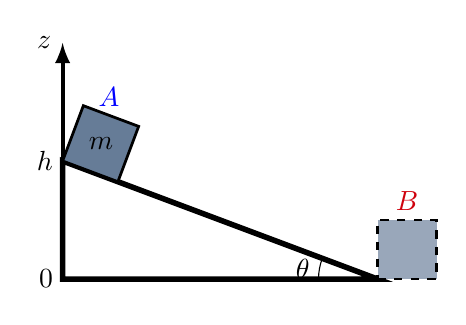
\begin{tikzpicture}[scale=1]
\tikzmath{
\L=4;
\h=1.5;
\abox=0.75;
\R=0.5*\abox;
\th=atan(\h/\L);
\d=\R+\L*cos(\th)/2;
}
\scalebox{1.0}{
\coordinate (Pb1) at (0,\h);%coordinates of box
\coordinate (Pb2) at ($(Pb1)+(-\th:\abox)$);
\coordinate (Pb3) at ($(Pb2)+(90-\th:\abox)$);
\coordinate (Pb4) at ($(Pb3)+(180-\th:\abox)$);
\coordinate (Pc) at (-\R,\h+\R);

\draw[-latex,line width=1.5] (0,0) -- (0,2*\h) node[left] {$z$};
\node[left] at (0,0) {$0$};
\node[left] at (0,\h) {$h$};

%plane and angle
\draw[line width=2pt] (0,\h) -- (0,0) -- (\L,0) -- cycle;
\draw (\L-0.75,0) arc(180:180-\th:0.75) node[midway,left]{$\theta$};


%rotated box
\draw[fill=myblue!60, line width=1] (Pb1) -- (Pb2) -- (Pb3) -- (Pb4) -- cycle ;
\node[color=blue] at ($(Pb3)+(-\abox/2,\abox/2)$) {$A$};
\node at ($(Pb1)+(45-\th:\abox/1.4)$) {$m$};

%box on the ground:
\draw[fill=myblue!40, dashed, line width=1] (1.0*\L,0) -- (1.0*\L+\abox,0) -- (1.0*\L+\abox,\abox) -- (1.0*\L,\abox) -- cycle;
\node[above,color=myred] at (1.0*\L+0.5*\abox,\abox) {$B$};

}
\end{tikzpicture}
\captionof*{figure}{\textit{A block slides down an incline with friction.}}
\end{center}
\scriptsize
\only<2->{
\begin{align*}
U(z)&=mgz\\
\textcolor{blue}{E_A=mgh} \;\;&\text{and}\;\; \textcolor{myred}{E_B=\frac{1}{2}mv^2}\\
W^{NC}&=-f_k\frac{h}{\sin\theta}\\
\therefore -f_k\frac{h}{\sin\theta} &= \textcolor{myred}{\frac{1}{2}mv^2} - \textcolor{blue}{mgh}\\
\only<3>{
\textcolor{myred}{\frac{1}{2}mv^2} &=\textcolor{blue}{mgh}-f_k\frac{h}{\sin\theta}
}
\end{align*}
}
}


%%%%%%%%%%%%%%%%%%%%%%%%%%%%%%%%
\twocolframesf{Conservation of energy}
{

\begin{itemize}
\item We can think of friction as increasing the ``thermal energy'' of the block (it heats up), $Q$, and include an additional type of energy.
\item In general we can think of $W^{NC}$ as some external agent injecting or removing energy, it doesn't have to be mechanical work and we can always account for it in terms of an energy.
\item If we include thermal energy in the system to model friction:
\begin{itemize}
\item All remaining forces are conservative.
\item Energy is always conserved.
\item We should include the incline into our ``system'' since it will share the heat with the block.
\end{itemize}
\end{itemize}

}
{
\vspace{-1.5cm}
\begin{center}
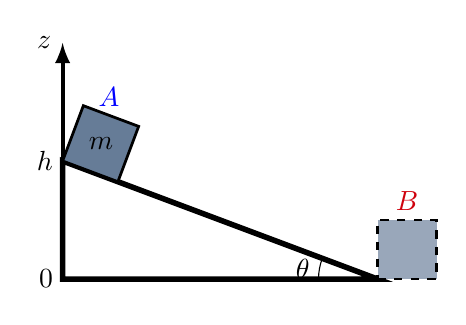
\begin{tikzpicture}[scale=1]
\tikzmath{
\L=4;
\h=1.5;
\abox=0.75;
\R=0.5*\abox;
\th=atan(\h/\L);
\d=\R+\L*cos(\th)/2;
}
\scalebox{1.0}{
\coordinate (Pb1) at (0,\h);%coordinates of box
\coordinate (Pb2) at ($(Pb1)+(-\th:\abox)$);
\coordinate (Pb3) at ($(Pb2)+(90-\th:\abox)$);
\coordinate (Pb4) at ($(Pb3)+(180-\th:\abox)$);
\coordinate (Pc) at (-\R,\h+\R);

\draw[-latex,line width=1.5] (0,0) -- (0,2*\h) node[left] {$z$};
\node[left] at (0,0) {$0$};
\node[left] at (0,\h) {$h$};

%plane and angle
\draw[line width=2pt] (0,\h) -- (0,0) -- (\L,0) -- cycle;
\draw (\L-0.75,0) arc(180:180-\th:0.75) node[midway,left]{$\theta$};


%rotated box
\draw[fill=myblue!60, line width=1] (Pb1) -- (Pb2) -- (Pb3) -- (Pb4) -- cycle ;
\node[color=blue] at ($(Pb3)+(-\abox/2,\abox/2)$) {$A$};
\node at ($(Pb1)+(45-\th:\abox/1.4)$) {$m$};

%box on the ground:
\draw[fill=myblue!40, dashed, line width=1] (1.0*\L,0) -- (1.0*\L+\abox,0) -- (1.0*\L+\abox,\abox) -- (1.0*\L,\abox) -- cycle;
\node[above,color=myred] at (1.0*\L+0.5*\abox,\abox) {$B$};

}
\end{tikzpicture}
\captionof*{figure}{\textit{A block slides down an incline with friction.}}
\end{center}
\scriptsize

\begin{align*}
\textcolor{myred}{Q_B}&=\textcolor{myred}{f_k\frac{h}{\sin\theta}}\\
\textcolor{blue}{E_A}&=\textcolor{blue}{mgh} \\
\textcolor{myred}{E_B}&=\textcolor{myred}{\frac{1}{2}mv^2+Q_B} \\
W^{NC}=0 \;\;&\rightarrow E_B=E_A\\
\therefore \textcolor{myred}{\frac{1}{2}mv^2+f_k\frac{h}{\sin\theta}} &=\textcolor{blue}{mgh}
\end{align*}

}

%%%%%%%%%%%%%%%%%%%%%%%%%%%%%%%%


%%%%%%%%%%%%%%%%%%%%%%%%%%%%%%%%










%%%%%%%%%%%%%%%%%%%%%%%%%%%%%%%

\section{Modelling Potential}
\label{sec:modelingpotential}
\title{Modeling Potential}
\institute{Conservation, Potential and Potential Uses}
\author{\insertsubsection}


%%%%%%%%%%%%%%%%%%%%%%%%%
\begin{frame}
\titlepage
\thispagestyle{empty}
\end{frame}

%%%%%%%%%%%%%%%%%%%%%%%%%%%%%%%%













%%%%%%%%%%%%%%%%%%%%%%%%%%%%%%%%
\subsection{Conservation of mechanical energy}
\label{subsec:conservationofmechanicalenergy}
\begin{frame}{Conservation of mechanical energy}
\begin{itemize}
\item When there is no net work being done by non-conservative forces, the mechanical energy is constant:
\begin{align*}
E&=\text{const.}=E_A=A_B\\
\Delta E&= 0 =\Delta U + \Delta K
\end{align*}
\item Potential and Kinetic energy ``trade off'' with each other:
\begin{align*}
\Delta K = -\Delta U
\end{align*}
\item If the potential energy increases, the kinetic energy must decrease by the same amount, and vice versa, \textit{just like the pendulum}.
\end{itemize}
\end{frame}


%%%%%%%%%%%%%%%%%%%%%%%%%%%%%%%%
\subsection{Example: marble on a track}
\label{subsec:marbleonatrackexample}
\twocolframesf{Example: marble on a track}
{
\begin{itemize}
\item If I place a marble on a track, it will move under the influence of gravity.
\item If I place it higher, it will have more initial energy, $E$.
\item The height at which I place it is a measure of its total energy, $E$ (it's all potential energy when I place the marble at rest).
\item As the marble rolls along the track, it will trade off kinetic and potential energy.
\end{itemize}
}
{
\begin{center}
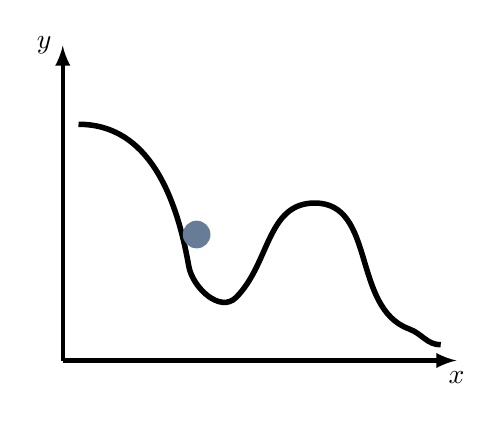
\begin{tikzpicture}
\tikzmath{
\L=4;
}

\scalebox{1}{

\draw[line width=1.5,-latex] (0,0) -- (1.25*\L,0) node[below] {$x$};
\draw[line width=1.5,-latex] (0,0) -- (0,\L) node[left] {$y$};

\draw[line width = 2]  (0.05*\L,0.75*\L) to [out=0,in=100] (0.4*\L,0.3*\L)  to [out=-80,in=225] (0.55*\L,0.2*\L) to [out=45,in=180] (0.8*\L,0.5*\L) to [out=0,in=160] (1.1*\L,0.1*\L) to [out=-20,in=180] (1.2*\L,0.05*\L);

\fill[myblue!60] ($(0.4*\L,0.3*\L)+(0.025*\L,0.1*\L)$) circle(5pt);

}

\end{tikzpicture}
\captionof*{figure}{\textit{A marble on a track in the vertical-horizontal plane.}}
\end{center}

}




%%%%%%%%%%%%%%%%%%%%%%%%%%%%%%%%
\twocolframesf{Example: marble on a track}
{
\begin{itemize}
\item The track \textbf{is} the gravitational potential energy as a function of horizontal position:
\begin{align*}
U(x)=mgy(x)\propto y(x)
\end{align*}
\item The initial ``height'' of the marble is the energy of the marble.
\item A potential energy function is like a track!
\item The energy of the marble is constant:
\begin{align*}
E&=U(x)+K\\
K&=E-U(x)
\end{align*}
\end{itemize}
}
{
\begin{center}
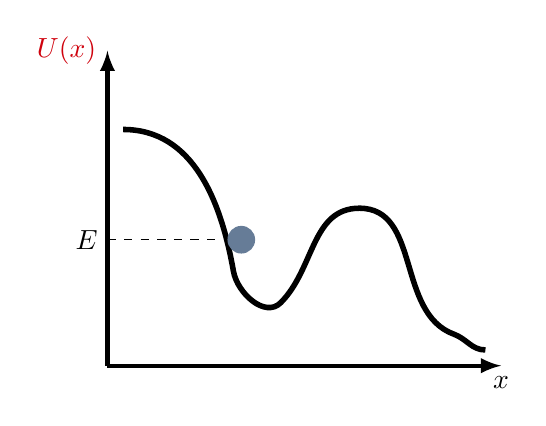
\begin{tikzpicture}
\tikzmath{
\L=4;
}

\scalebox{1}{

\draw[line width=1.5,-latex] (0,0) -- (1.25*\L,0) node[below] {$x$};
\draw[line width=1.5,-latex] (0,0) -- (0,\L) node[left] {\textcolor{myred}{$U(x)$}};

\draw[line width = 2]  (0.05*\L,0.75*\L) to [out=0,in=100] (0.4*\L,0.3*\L)  to [out=-80,in=225] (0.55*\L,0.2*\L) to [out=45,in=180] (0.8*\L,0.5*\L) to [out=0,in=160] (1.1*\L,0.1*\L) to [out=-20,in=180] (1.2*\L,0.05*\L);

\draw[dashed] ($(0,0.3*\L)+(0,0.1*\L)$) node[left]{$E$} -- ($(0.4*\L,0.3*\L)+(0.025*\L,0.1*\L)$);
\fill[myblue!60] ($(0.4*\L,0.3*\L)+(0.025*\L,0.1*\L)$) circle(5pt);

}

\end{tikzpicture}
\captionof*{figure}{\textit{In 1D, the potential energy function can be thought of as a track for a marble.}}
\end{center}

}


%%%%%%%%%%%%%%%%%%%%%%%%%%%%%%%%
\subsection{Potential energy for a spring}
\label{subsec:potentialenergyforaspring}
\begin{frame}{Potential energy for a spring}
We can interpret any potential energy function as if it were a track upon which we put a marble.
\begin{align*}
U(x)=\frac{1}{2}kx^2
\end{align*}

\begin{columns}[T]
 \column{0.5\textwidth}
 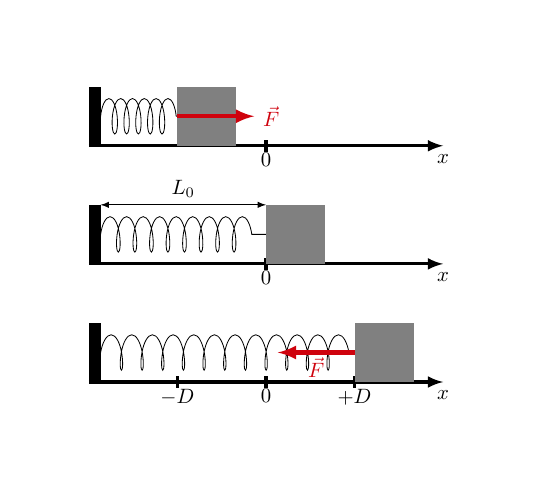
\begin{tikzpicture}[scale=1]
\tikzmath{
\L=2.;
\dx=0.75*\L;
\off=0.5;
\h=1;
}
\scalebox{0.75}{


\draw[-latex,line width=1.5pt] (-1.5*\L,0) -- (1.5*\L,0) node[below]{$x$};
\draw[line width=1.5pt] (0,-0.1) -- (0,0.1);
\node[below] at (0,0) {$0$};

\fill (-1.5*\L,0) rectangle (-1.4*\L,\h);
\draw[decoration={aspect=0.3, segment length=2.8mm, amplitude=3mm,coil},decorate] (-1.4*\L,\h/2) -- (0,\h/2);
\draw [latex-latex] (-1.4*\L,\h) -- (0,\h) node[midway,above]{$L_0$};
\fill[black!50] (0,0) rectangle (\h,\h);

%%%%%%%%%%  top compressed
\begin{scope}[shift={(0,2*\h)}]
\draw[-latex,line width=1.5pt] (-1.5*\L,0) -- (1.5*\L,0) node[below]{$x$};
\draw[line width=1.5pt] (0,-0.1) -- (0,0.1);
\node[below] at (0,0) {$0$};

\fill (-1.5*\L,0) rectangle (-1.4*\L,\h);
\draw[decoration={aspect=0.3, segment length=2mm, amplitude=3mm,coil},decorate] (-1.4*\L,\h/2) -- (-\dx,\h/2);
\fill[black!50] (-\dx,0) rectangle (-\dx+\h,\h);
\draw[line width=2, -latex, color=myred] (-\dx,\h/2) -- +(1.3,0) node[right] {$\vec F$};

\end{scope}
%%%%%%%%%% bottom extended
\begin{scope}[shift={(0,-2*\h)}]
\draw[-latex,line width=1.5pt] (-1.5*\L,0) -- (1.5*\L,0) node[below]{$x$};
\node[below] at (-\dx,0){$-D$};
\draw[line width =1.5pt] (-\dx,0.1) -- +(0,-0.2);
\node[below] at (\dx,0){$+D$};
\draw[line width =1.5pt] (\dx,0.1) -- +(0,-0.2);
\draw[line width=1.5pt] (0,-0.1) -- (0,0.1);
\node[below] at (0,0) {$0$};

\fill (-1.5*\L,0) rectangle (-1.4*\L,\h);
\draw[decoration={aspect=0.3, segment length=3.5mm, amplitude=3mm,coil},decorate] (-1.4*\L,\h/2) -- (\dx,\h/2);
\fill[black!50] (\dx,0) rectangle (\dx+\h,\h);
\draw[line width=2, -latex, color=myred] (\dx,\h/2) -- +(-1.3,0) node[midway,below=-2pt] {$\vec F$};
\end{scope}

}
\end{tikzpicture}
 
 
 \column{0.5\textwidth}
 \vspace{-1.2cm}
 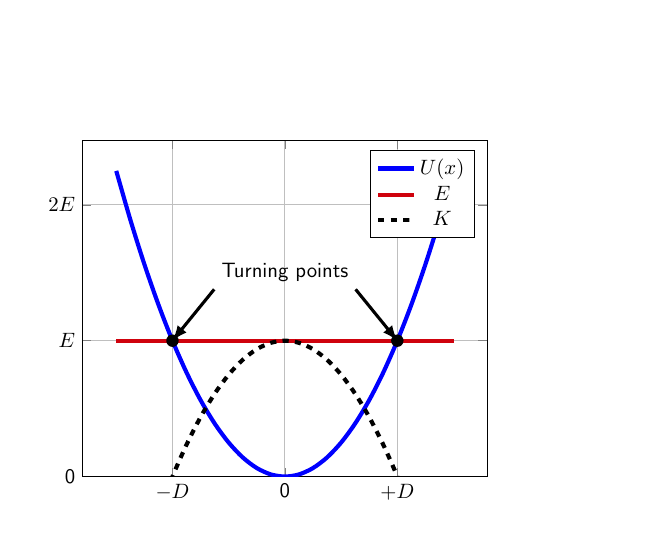
\begin{tikzpicture}
 \scalebox{0.75}{
 \begin{axis}[domain = -3:3, ymin=0,legend pos=north east,
              grid, xtick = {-2, 0, 2}, xticklabels = {$-D$, 0, $+D$}, ytick = {0, 8, 16}, yticklabels = {0, $E$, $2E$}]
  \addplot[smooth,color=blue,line width=2] {2*x^2};
  \addplot[smooth,color=myred,line width=2] {8};
  \addplot[smooth,dashed,line width=2] {8-2*x^2};
  \addlegendentry{$U(x)$}
  \addlegendentry{$E$}
  \addlegendentry{$K$}
  
  \fill[coordinate] (axis cs:-2,8) circle(3pt);
  \fill[coordinate] (axis cs:2,8) circle(3pt);
  
  \node (label) at (axis cs:0,12)  {Turning points};
  \draw[-latex,line width=1.5pt] (label.south west) -- (axis cs:-2,8);
  \draw[-latex,line width=1.5pt] (label.south east) -- (axis cs:2,8);
 \end{axis}

 }
 \end{tikzpicture}
 
 \end{columns}
\end{frame}


%%%%%%%%%%%%%%%%%%%%%%%%%%%%%%%%


%%%%%%%%%%%%%%%%%%%%%%%%%%%%%%%%
\subsection{How to model with energy}
\label{subsec:howtomodelwithenergy}
\begin{frame}{Modeling with energy (how to)}
\begin{itemize}
\item The most important step is \sout{identifying the forces} identifying the potential energies and sources of non-conservative work.
\item Compare energy at some point (time) A and some other point (time) B; the difference in mechanical energies is the work done by non-conservative forces:
\begin{align*}
E_A&=K_A+U_{1A}+U_{2A}+\dots\\
E_B&=K_B+U_{1B}+U_{2B}+\dots\\
\rightarrow W^{NC}&=E_B-E_A
\end{align*}
\end{itemize}

\end{frame}


%%%%%%%%%%%%%%%%%%%%%%%%%%%%%%%%
\subsection{Intro to The Lagrangian}
\label{subsec:introtothelagrangian}
\begin{frame}{The Lagrangian: A completely different approach}
\begin{itemize}
\item You won’t be tested on your knowledge of this, however...
\item It is presented to you as a different way to build models:
\begin{itemize}
\item We give you a prescription and tell you that if you follow those rules, you will develop a model that describes the world.
\item You should be open to that process (following rules, not understanding the rules – nobody can seriously claim to fully understand them).
\end{itemize}

\item The Lagrangian method is very powerful, carries into Quantum Mechanics, and is mathematically very aesthetic. It almost feels as if there is an underlying beauty to it all...
\end{itemize}
\end{frame}


%%%%%%%%%%%%%%%%%%%%%%%%%%%%%%%%
\subsubsection{Structure}
\label{subsubsec:structurelagrangian}
\twocolframe{The prescription}
{
\begin{enumerate}
\item Build the Lagrangian:
\begin{align*}
L=K-U
\end{align*}
\item Apply the Euler-Lagrange equation:
\begin{align*}
\frac{d}{dt}\left( \frac{\partial L}{\partial v_x} \right) - \frac{\partial L}{\partial x} =0
\end{align*}
\end{enumerate}
This gives the equations of motion (e.g. the acceleration).\\
You get one such equation per coordinate (e.g. replace $(x,v_x)$ with $(y, v_y)$ if these also appear in $L$).
}
{
\only<2>{
For a particle falling with gravity ($x$ positive upwards):
\begin{align*}
L&=\frac{1}{2}mv^2-mgx\\
\frac{d}{dt}\left( \frac{\partial L}{\partial v_x} \right) &=\frac{d}{dt}\left(mv \right) = ma\\
\frac{\partial L}{\partial x} &= -mg\\
\therefore ma + mg&=0\\
a&=-g
\end{align*}
As expected, the acceleration is $-g$, since $x$ is positive upwards.

 }

}


%%%%%%%%%%%%%%%%%%%%%%%%%%%%%%%%
\subsubsection{Lagrangian for a pendulum}
\label{subsubsec:lagrangianforapendulum}
\twocolframesf{Lagrangian for a pendulum}
{
For a pendulum, we use the angle $\theta$ as the coordinate to describe position. The speed is given by $v=\omega L$, where $\omega=\frac{d\theta}{dt}$:
\begin{align*}
K&=\frac{1}{2}mv^2=\frac{1}{2}mL^2\omega^2\\
U&=mgh=mgL(1-\cos\theta)\\
\therefore L&=K-U=\frac{1}{2}mL^2\omega^2-mgL(1-\cos\theta)
\end{align*}
The Euler-Lagrange equation is:
\begin{align*}
\frac{d}{dt}\left( \frac{\partial L}{\partial \omega} \right) - \frac{\partial L}{\partial \theta} =0
\end{align*} 
}
{
\vspace{-0.75cm}
\begin{center}
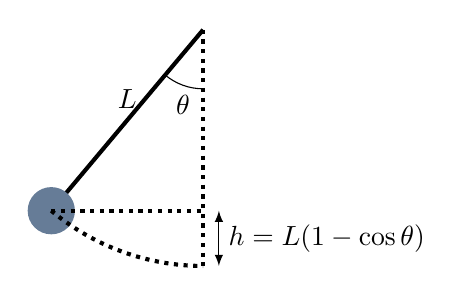
\begin{tikzpicture}[scale=1]
\tikzmath{
\L=3.;
\R=0.3;
\th=40;
\vg=1;
\Ly=\L*cos(\th);
}
\scalebox{1.0}{
%pendulum

\draw[line width = 1.5pt] (0,0) -- (270-\th:\L) node[midway,above]{$L$};
\fill[color=myblue!60] (270-\th:\L) circle(\R); 

\draw[dotted, line width = 1.5pt] (0,0) -- (270:\L);
\draw[dotted, line width = 1.5pt] (270-\th:\L) arc (270-\th:270:\L);
\draw (270-\th:0.75) arc (270-\th:270:0.75) node[midway,below]{$\theta$};
\draw[dotted, line width = 1.5pt] (270-\th:\L) -- (0,-\Ly);
\draw[latex-latex] (0.2,-\L) -- (0.2,-\Ly) node[midway,right]{$h=L(1-\cos\theta)$};
}
\end{tikzpicture}
\end{center}
\only<2>{
\begin{align*}
\frac{d}{dt}\left( \frac{\partial L}{\partial \omega} \right) = \frac{d}{dt}\left( mL^2\omega \right)&=mL^2\alpha\\
\frac{\partial L}{\partial \theta} &=-mgL\sin\theta\\
\therefore mL^2\alpha + mgL\sin\theta&=0\\
\alpha &=\frac{g}{L}\sin\theta
\end{align*}
}
}


%%%%%%%%%%%%%%%%%%%%%%%%%%%%%%%%
\subsubsection{Noether's Theorem}
\label{subsubsec:noethertheorem}
\twocolframesf{Emmy Noether's theorem}
{
\begin{itemize}
\item If the Lagrangian is ``invariant to some symmetry'', then something is conserved.
\item This ties the idea of a conserved quantity to some symmetry in the laws of nature.
\item For example, if the Lagrangian does not change with time, then energy is conserved.
\item We now see conservation laws as the result of symmetries in the laws of physics.
\item Momentum, charge, energy are conserved because the laws of physics are invariant to different ``symmetries''. 
\end{itemize}
}
{\vspace{-0.5cm}
\capfig{0.7}{figures/PotentialECons/noether}{Emmy Noether. (2025, August 12). Wikipedia, the free encyclopedia. Retrieved August 25, 2025, from https://en.wikipedia.org/wiki/Emmy\_Noether}
}  
  

%%%%%%%%%%%%%%%%%%%%%%%%%%%%%%%%
\subsection{The Standard Model of particle physics}
\label{subsec:thestandardmodelofparticlephysics}
\twocolframesf{The Standard Model of particle physics}
{
\begin{itemize}
\item The Standard Model of Particle physics describes the three forces (weak, strong, e/m) of nature that are not gravity. It’s just a Lagrangian.
\item Each term represents some interaction between particles.
\item Only certain functional forms are allowed in order to preserve symmetries.
\item So far, it appears that every (mathematically) allowable term describes something in nature. That’s pretty cool.
\item People have discovered particles based on the idea that a particular term could be present in the Lagrangian. 
\end{itemize}
}
{
\capfig{1.1}{figures/PotentialECons/LSM}{The Lagrangian for the Standard Model.}
} 


%%%%%%%%%%%%%%%%%%%%%%%%%%%%%%%%


%%%%%%%%%%%%%%%%%%%%%%%%%%%%%%%%



%%%%%%%%%%%%%%%%%%%%%%%%%%%%%%%%



%%%%%%%%%%%%%%%%%%%%%%%%%%%%%%%%



%%%%%%%%%%%%%%%%%%%%%%%%%%%%%%%%



%%%%%%%%%%%%%%%%%%%%%%%%%%%%%%%%






\end{document}







